
\documentclass{standalone}
\usepackage{pgfplots}
\usepackage{verbatim}
\usepackage{tikz}
\usepackage{pgfplots}
%\usepackage{pgfmath}
\usetikzlibrary{patterns}
\usetikzlibrary{shapes}
\usetikzlibrary{arrows}
%minimum size=10pt, inner sep=0pt

\begin{document}
\newcommand{\ptfont}[1]{\fontsize{#1}{\baselineskip}\selectfont}
\newcommand{\labelfont}{25pt}
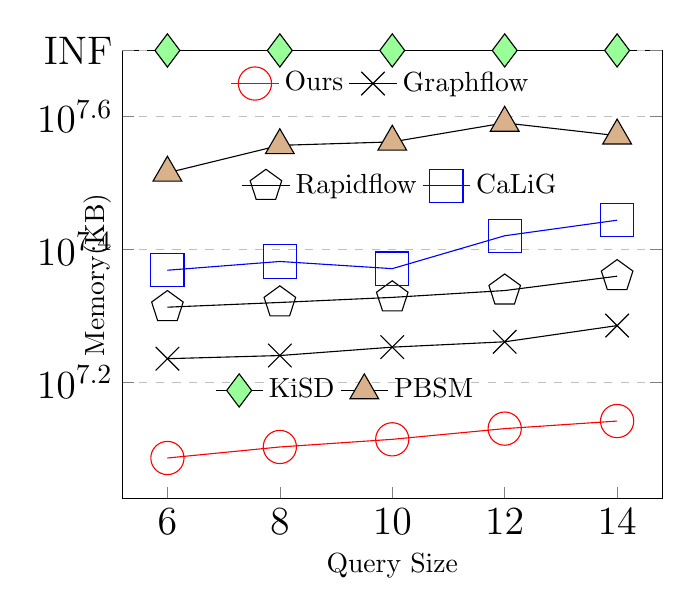
\begin{tikzpicture}
\newenvironment{customlegend}[1][]{%
    \begingroup
    % inits/clears the lists (which might be populated from previous
    % axes):
    \csname pgfplots@init@cleared@structures\endcsname
    \pgfplotsset{#1}%
}{%
    % draws the legend:
    \csname pgfplots@createlegend\endcsname
    \endgroup
}%

% makes \addlegendimage available (typically only available within an
% axis environment):
\def\addlegendimage{\csname pgfplots@addlegendimage\endcsname}
\def\addlegendentry{\csname pgfplots@addlegendentry\endcsname}

\tikzstyle{mymarksize} = [mark size=6pt]

%for 2023vldb
\tikzstyle{ourMark} = [color=red,mark=o,mymarksize]
\tikzstyle{graphflowMark} = [color=black,mark=x,mymarksize]
\tikzstyle{caligMark} = [color=blue,mark=square,  mymarksize]
\tikzstyle{rapidflowMark} = [color=black,mark=pentagon,mymarksize]
\tikzstyle{instopkMark} = [color=black,mark=diamond*,mymarksize,mark options={solid, fill=green!40},mymarksize]
\tikzstyle{pbsmMark} = [color=black,mark=triangle*,mark options={solid, fill=brown!60,only marks},mymarksize]

% \tikzstyle{globalMark} = [color=black,mark=star, mark options={solid, fill=black!30}, mymarksize]
% \tikzstyle{localMark} = [color=blue,mark=square,  mymarksize]
% \tikzstyle{candidateMark} = [color=black!40!green,mark=triangle,mymarksize]
% \tikzstyle{edgeMark} = [color=black,mark=otimes,mymarksize]
% \tikzstyle{graphflowPlusMark} = [color={rgb:red,4;black,2;yellow,1},mark=diamond,mymarksize]
% \tikzstyle{symbiMark} = [color=black,mark=otimes,mymarksize]
% \tikzstyle{turboMark} = [color=black,mark=diamond*,mymarksize,mark options={solid, fill=green!40}]
% \tikzstyle{graphflowMark} = [color=black,mark=triangle*,mark options={solid, fill=brown!60,only marks},mymarksize]

%for barfill
\tikzstyle{ourfill} = [color=black,fill=red!40,]
\tikzstyle{edgeindexfill} = [color=black, fill=green!20,postaction={pattern=grid}]
\tikzstyle{globalindexfill} = [color=black, fill=blue!20, postaction={pattern=crosshatch dots}]
\tikzstyle{localindexfill} = [color=black, pattern = north west lines]
%caseStudy
\tikzstyle{itopkfill} = [color=black,fill=yellow, postaction={pattern=north east lines}]
\tikzstyle{pbsmfill} = [color=black, fill=green!20, postaction={pattern=crosshatch dots}]
\tikzstyle{dsmfill} = [color=black,fill=red!40 ,postaction={pattern=grid}]

%counterparts
 \tikzstyle{graphflowfill} = [color=black,fill=blue!20 ,postaction={pattern=crosshatch}]
\tikzstyle{globalfill} = [color=black,fill=yellow, postaction={pattern=north east lines}]
\tikzstyle{localfill} = [color=black, fill=green!20, postaction={pattern=crosshatch dots}]
\tikzstyle{dsmfill} = [color=black,fill=red!40 ,postaction={pattern=grid}]

%vary query size
\tikzstyle{q6Mark} = [color=black,mark=*,mark options={fill=black!30},mymarksize]
\tikzstyle{q8Mark} = [color=black, mark=square*, mymarksize, mark options={solid, fill=blue!30}]
\tikzstyle{q10Mark} = [color=black,mark=otimes,mark options={solid,fill=yellow!40},mymarksize]
\tikzstyle{q12Mark} = [color=black,mark=diamond*,mymarksize,mark options={solid, fill=green!40}]
\tikzstyle{q14Mark} = [color=black,mark=triangle*,mark options={solid, fill=brown!60,only marks},mymarksize]

% insertion and deletion distribute
\tikzstyle{deletionfill} = [color=black, fill=green!20, postaction={pattern=crosshatch dots}]
\tikzstyle{insertionfill} = [color=black,fill=yellow, postaction={pattern=north east lines}]

% insertion and deletion Ratio
\tikzstyle{k100fill} = [color=black, fill=black]
\tikzstyle{k300fill} = [color=black,fill=gray!40,postaction={pattern=dots}]
\tikzstyle{k500fill} = [color=black, fill=blue!40,postaction={pattern=north east lines}]
\tikzstyle{k700fill} = [color=black,fill=green!20, postaction={pattern=fivepointed stars}]
\tikzstyle{k900fill} = [color=black,fill=red!40,postaction={pattern=crosshatch dots}]

%compressRatio
% insertion and deletion Ratio
\tikzstyle{q6fill} = [color=black, fill=black]
\tikzstyle{q8fill} = [color=black,fill=gray!40,postaction={pattern=dots}]
\tikzstyle{q10fill} = [color=black, fill=blue!40,postaction={pattern=north east lines}]
\tikzstyle{q12fill} = [color=black,fill=green!20, postaction={pattern=fivepointed stars}]
\tikzstyle{q14fill} = [color=black,fill=red!40,postaction={pattern=crosshatch dots}]

%for index construction
\tikzstyle{indexOurMark} = [color=black, fill=black]
\tikzstyle{indexRapifFlow} = [color=black,fill=gray!40,postaction={pattern=dots}]
\tikzstyle{indexCaLig} = [color=black, fill=blue!40,postaction={pattern=north east lines}]
\tikzstyle{indexIsoTopk} = [color=black,fill=green!20, postaction={pattern=fivepointed stars}]
\tikzstyle{indexPBSM} = [color=black,fill=red!40,postaction={pattern=crosshatch dots}]

%couterparts mymarksize
% \tikzstyle{globalMark} = [color=black,mark=star, mark options={solid, fill=black!30}, ]
% \tikzstyle{localMark} = [color=blue,mark=square,  mymarksize]
% \tikzstyle{ourMark} = [color=black!40!red,mark=triangle,mymarksize]
% \tikzstyle{baselineMark} = [color=black,mark=otimes,mymarksize]

% \tikzstyle{globalMark} = [color=black, mark=star, mark options={solid, fill=black!50}, mymarksize, line width=0.6pt]
% \tikzstyle{localMark} = [color=blue, mark=o, mark options={solid, fill=blue!30, scale=0.7}, mymarksize, line width=0.6pt]
% \tikzstyle{ourMark} = [color=red, mark=triangle, mark options={solid, fill=red!50},mymarksize,line width=0.6pt]
% \tikzstyle{baselineMark} = [color=black,mark=diamond*,mymarksize,mark options={solid, fill=green!40},mark size=3pt]

% %for linemark
% \tikzstyle{ourMark} = [color=red,mark=o,mymarksize]
% \tikzstyle{sjMark} = [color=black,mark=x,mymarksize]
% \tikzstyle{boostMark} = [color=blue,mark=square,  mymarksize]
% \tikzstyle{vf2Mark} = [color=black!40!green,mark=triangle,mymarksize]
% \tikzstyle{nomsMark} = [color={rgb:red,4;black,2;yellow,1},mark=diamond,mymarksize]
% %\tikzstyle{turboMark} = [color=black,mark=otimes,mymarksize]
% \tikzstyle{vf2colorMark} = [color=black,mark=diamond*,mymarksize,mark options={solid, fill=green!40}]
% \tikzstyle{quicksiMark} = [color=black,mark=triangle*,mark options={solid, fill=brown!60,only marks},mymarksize]
% \tikzstyle{dpmark} = [color=black,mark=10-pointed star,mymarksize]
% \tikzstyle{rlismark} = [color=black,mark=star, mark options={solid, fill=black!30}, mymarksize]


% \tikzstyle{netMark} = [color=red,mark=o,mymarksize]
% \tikzstyle{rdfMark} = [color=black,mark=x,mymarksize]
% \tikzstyle{wktMark} = [color=blue,mark=square,mymarksize]

% \tikzstyle{concuroneMark} = [color=red, mark=o,mymarksize]
% \tikzstyle{concurtwoMark} = [color=red, mark=x,mymarksize]
% \tikzstyle{concurthrMark} = [color=red, mark=square,  mymarksize]
% \tikzstyle{concurforMark} = [color=red, mark=triangle,mymarksize]
% \tikzstyle{concurfivMark} = [color=red, mark=diamond,mymarksize]

% \tikzstyle{pessimoneMark} = [color=black, mark=o,mymarksize]
% \tikzstyle{pessimtwoMark} = [color=black, mark=x, mymarksize]
% \tikzstyle{pessimthrMark} = [color=black,mark=square,mymarksize]
% \tikzstyle{pessimforMark} = [color=black,mark=triangle,mymarksize]
% \tikzstyle{pessimfivMark} = [color=black,mark=diamond, mark options={solid, fill=black!30}, mymarksize]

% %for barfill

% \tikzstyle{ourfill} = [fill=black]
% \tikzstyle{rapidFlowfill} = [color=black, pattern=dots]
% \tikzstyle{baseline3fill} = [color=black,fill=blue!40 ,postaction={pattern=crosshatch}]
% \tikzstyle{baseline2fill} = [color=black,pattern = north west lines]
% \tikzstyle{baseline1fill} = [color=black, fill=black!3]
% \tikzstyle{graphflowPlusfill} = [color=black, fill=black!30]
% \tikzstyle{graphflowfill} = [color=black,fill=yellow, postaction={pattern=north east lines}]
% \tikzstyle{symbifill} = [color=black, fill=green!20, postaction={pattern=fivepointed stars}]
% \tikzstyle{turbofill} = [color=black,fill=red!40 ,postaction={pattern=grid}]
% \tikzstyle{rlisfill} = [color=black,fill=blue!40 ,postaction={pattern=crosshatch}]
% \tikzstyle{lisonefill} = [color=black, fill=black!20, postaction={pattern=dots}]

%for x tick
\def\drone{10}
\def\drtwo{20}
\def\drthr{30}
\def\drfor{40}
\def\drfiv{50}

\def\qszone{6}
\def\qsztwo{9}
\def\qszthr{12}
\def\qszfor{15}
\def\qszfiv{18}
\def\qszsix{21}

%\def\pone{0.00}
%\def\ptwo{0.25}
%\def\pthr{0.50}
%\def\pfor{0.75}
%\def\pfiv{1.00}
%\def\psix{10}

\def\pone{1}
\def\ptwo{3}
\def\pthr{6}
\def\pfor{9}
\def\pfiv{12}
\def\psix{15}

\def\gNumone{6}
\def\gNumtwo{8}
\def\gNumthr{10}
\def\gNumfor{12}
\def\gNumfiv{14}

\def\gKNumone{100}
\def\gKNumtwo{300}
\def\gKNumthr{500}
\def\gKNumfor{700}
\def\gKNumfiv{900}

\def\gSizeone{6}
\def\gSizetwo{8}
\def\gSizethr{10}
\def\gSizefor{12}
\def\gSizefiv{14}
\def\gSizesix{16}

\def\dataSetone{Amazon}
\def\dataSettwo{LiveJournal}
\def\dataSetthr{Human}
\def\dataSetfor{Youtube}

\def\qNumone{20}
\def\qNumtwo{40}
\def\qNumthr{60}
\def\qNumfor{80}

% compare function
\def\ctk{Ours}
\def\gf{Graphflow}
\def\rf{Rapidflow}
\def\cg{CaLiG}
\def\itk{KiSD}
\def\pm{PBSM}

%database
\def\az{Amazon}
\def\lj{Livejournal}
\def\hn{Human}
\def\ytb{Youtube}

% fixqueryszie distrbution
\tikzstyle{onefill} = [fill=black]
\tikzstyle{twofill} = [color=black,fill=white,postaction={pattern=dots}]
%[color=black, pattern=dots]
\tikzstyle{thrfill} = [color=black,fill=white,postaction={pattern=north west lines}]
%[color=black, pattern = north west lines]
\tikzstyle{forfill} = [color=black,fill=white,postaction={pattern=grid}]
%[color=black, fill=black!30]
\tikzstyle{fivfill} = [color=black, postaction={pattern=north east lines}]
%[color=black, fill=black!30]
%\tikzstyle{varIDfill} = [color=black,fill=yellow, postaction={pattern=north east lines}]
\tikzstyle{sixfill} = [color=blue, postaction={pattern=dots}]



\def\scorewid{30}
\def\scorehgt{10}

% counter parts
\newcommand{\couterpartslegend}{
    \legend{Our-final,MWstar-both,MWstar-global,Baseline}
}

\newcommand{\fixksizelegend}{
\legend{Ours, Graphflow,Rapidflow,CaLiG,KiSD,PBSM}
}
\newcommand{\fixksizecouterparts}{
\legend{Baseline, MWstar-global,MWstar-both,Our-final}
}


\begin{semilogyaxis}
[
    ymin = 0,
    ymax=50000000,
 %   ymax=0.9,
 %   xmin = 0,
 %   xmax =110
 %    width = 7cm,
 %    height = 6cm,
 %    nodes near coords,
     point meta=rawy,
     ymajorgrids = true,% add gridslines in ylabel
     grid style=dashed,
     ylabel = {Memory(KB)},
     %    scaled x ticks = base 10:-3,
     /pgf/number format/1000 sep={},
        xlabel = {Query Size},
                 xtick={\gNumone, \gNumtwo, \gNumthr, \gNumfor, \gNumfiv},
 %    ytick={0, 0.2, 0.4, 0.6, 0.8, 1.0},
 %    legend pos= north east,
     legend cell align=left,
     x label style = {font=\ptfont{\labelfont}},
     ticklabel style = {font=\Large},
     y label style = {inner sep=0pt,at={(axis description cs:-0.02,0.5)},font=\ptfont{\labelfont}},
     extra y ticks={50000000},
      extra y tick label={INF},
]

\addplot [ourMark]
coordinates {(\gNumone, 12183340 ) (\gNumtwo, 12658810 )  (\gNumthr,12998570)  (\gNumfor,13489210  )  (\gNumfiv,13847890  )};

\addplot [graphflowMark]
coordinates {(\gNumone, 17189490  ) (\gNumtwo, 17376380  )  (\gNumthr, 17889490 )  (\gNumfor, 18223940  )  (\gNumfiv,19276380  )};

\addplot [rapidflowMark]
coordinates {(\gNumone, 20545600 ) (\gNumtwo,20883439  )  (\gNumthr, 21254586  )  (\gNumfor, 21763321  )  (\gNumfiv, 22873421  )};

\addplot [caligMark]
coordinates {(\gNumone, 23350667.43  ) (\gNumtwo, 24069862.27  )  (\gNumthr, 23479422.95 )  (\gNumfor,  26311767.64  )  (\gNumfiv,27770294.87  )};

\addplot [instopkMark]
coordinates {(\gNumone, 50000000) (\gNumtwo,50000000 )  (\gNumthr, 50000000 )  (\gNumfor, 50000000 )  (\gNumfiv, 50000000 )};

\addplot [pbsmMark]
coordinates{(\gNumone, 32725400  ) (\gNumtwo, 35990485.92 )  (\gNumthr, 36428610.37  )  (\gNumfor, 38906904.7)  (\gNumfiv, 37221241.53  )};


\end{semilogyaxis}

% 31238.77117	29799.44212	32041.23502	19532.96765	18696.43799	17069.86616
%\addplot [vf2Mark]
%coordinates {(\qszone, 31238)  (\qsztwo, 29799)  (\qszthr, 32041)  (\qszfor, 19532)  (\qszfiv, 18696)  (\qszsix, 17069) };


% \fixNum
\begin{customlegend}[legend style={at={(3.55, 4.2) ,font=\ptfont{19pt}}, draw=none, row sep=-0.6pt, fill=none, anchor = north,inner sep = 0pt},legend columns = 2,legend cell align=left,legend entries={\rf,\cg}]
    \addlegendimage{rapidflowMark}
    \addlegendimage{caligMark}
\end{customlegend}

\begin{customlegend}[legend style={at={(3.3, 5.5) ,font=\ptfont{19pt}}, draw=none, row sep=-0.6pt, fill=none, anchor = north,inner sep = 0pt},legend columns = 2,legend cell align=left,legend entries={\ctk,\gf}]
    \addlegendimage{ourMark}
    \addlegendimage{graphflowMark}
\end{customlegend}


\begin{customlegend}[legend style={at={(2.85, 1.6) ,font=\ptfont{19pt}}, draw=none, row sep=-0.6pt, fill=none, anchor = north,inner sep = 0pt},legend columns = 2,legend cell align=left,legend entries={\itk,\pm}]
\addlegendimage{instopkMark}
\addlegendimage{pbsmMark} 
\end{customlegend}

% \begin{customlegend}[legend style={at={(4.35, 0.8) ,font=\ptfont{10pt}}, draw=none, row sep=-0.6pt, fill=none, anchor = north, inner sep = 0pt},legend columns = 2,legend cell align=left,legend entries={ }]
% \end{customlegend}

\end{tikzpicture}
\end{document}

